\documentclass{article}

\usepackage{fancyhdr}
\usepackage{mathtools}
\usepackage{amsmath}
\usepackage{amssymb}
\usepackage{amsfonts}
\usepackage{cases}
\pagestyle{fancy}

\author{
  Robin Touche \\
  \and
  Fredrik Bredmar
}

\title{Machine Learning Homework 5}

\begin{document}

\maketitle

\subsection*{1.1}
In this problem we analytically calculate the weight vector of the optimal hyperplane corresponding to a set of given points.
Figure one shows a plot of the given points.\\

The linear kernel describing our weight vector is defined as
\[
w_1x_1 + w_2*x_2 + b = 0
\]

By looking at the plot we see four points that will be support vectors.
If we take the distance between the two upper points, $(0,2)$ and $(2,2)$ we get that the point right between them is $(1,2)$.
If we do the same for the two lower points $(2,0)$ and $(4,0)$ we get the point $(3,0)$ right between them.
The points between the pairs of support vectors is all we need to compute the linear kernel for our weight vector. We setup an equation system of the points and solve it to get the weight vector.
The equation system looks as follows.
\[
\begin{cases}

  w_1  + 2w_2 &+ b = 0 \\
  3w_1 &+  b = 0

\end{cases}
\]
After solving the equation system we get

\[
\begin{cases}
w_1 = w_2\\
b = -3w_1
\end{cases}
\]
So a convenient solution is to set the weight vector to $w_1 = w_2 = 1$ and therefore $b=-3$.
With this solution we can now calculate the margin of the optimal hyperplane to the support vectors.
The distance is given by
\[
  \frac{|w_1a_1+w_2a_2+b |}{\sqrt{w_1^2+w_2^2}}
\]
Let $(a_1,a_2)$ be a support vector, for example $(2,0)$ and we get $\gamma = \frac{1}{\sqrt2}$.
So we get that the margin is $2\gamma = \sqrt2$.
\begin{figure}
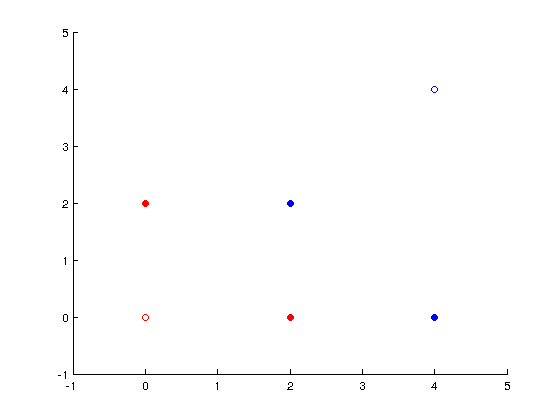
\includegraphics[scale=0.6]{pics/plot11.png}
\caption{Plot of the given points in problem 1.1.
  Red points are classified as -1 and blue points are classified as +1.
Filled points are support vectors.}
\end{figure}

\subsection*{1.2}
\paragraph{a}

We wish to find a solution to

\begin{align}
  arg \min_{(\mathbf{w}, b)} \frac{1}{2} \lvert \rvert \mathbf{w}^2 \lvert \rvert
\end{align}
subject to the constraint that for all $i = 1, ... , n$

\begin{align}
  y_i (\mathbf{w} \cdot x_i - b) \geq 1
\end{align}
Using the Lagrange multiplier method this can be expressed as

\begin{align}
  arg \min_{(\mathbf{w}, b)} \max_{a > 0} \left\{ \frac{1}{2} \lvert \rvert \mathbf{w}^2 \lvert \rvert -
      \sum_{i = 1}^{n}\alpha_i \big( y_i \left( \mathbf{w} \cdot x_i - b \right) - 1 \big) \right\}
\end{align}
Which can be simplified to

\begin{align}
  \mathbf{w} = \sum_{i = 1}^{n}\alpha_i y_i x_i
\end{align}

Only those $\alpha_i$ where $x_i$ is a support vector will be greater than
zero. These support vectors lie on the margin and will thus satisfy $y_i \left(
\mathbf{w} \cdot x_i - b \right) = 1$.

By reorganising the above equation we now have an expression for $b$. As $b$
depends on each data point we can just average over all the support vectors and
get

\begin{align}
  b = \frac{1}{N} \sum_{i = 1}^{N} \left( \mathbf{w} \cdot x_i - y_i \right)
\end{align}

where $N$ is the number of support vectors.


\subsection*{2.1}
\paragraph{a}
See code.

\paragraph{b}
See Figure 2.
\begin{figure}
\begin{center}
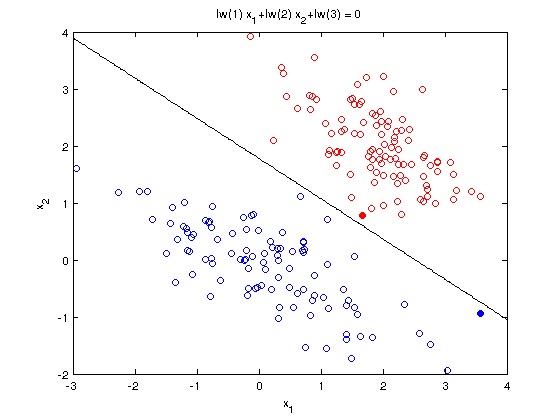
\includegraphics[scale = 0.6]{pics/plot21.png}
\caption{Plot for problem 2.1, the support vectors are marked as filled points.}
\end{center}
\end{figure}
\paragraph{c}
It has a bias of $\approx 1.7785$.

\paragraph{d}
The margin is $2\gamma \approx 0.3046$.

\subsection*{2.2}
\paragraph{a}
See Figure 3.
\begin{figure}
\begin{center}
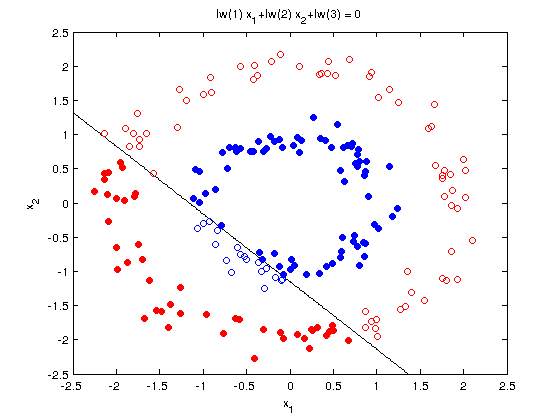
\includegraphics[scale = 0.6]{pics/plot22.png}
\caption{ Plot for problem 2.2, the filled points are correctly classified.}
\end{center}
\end{figure}

\paragraph{b}

Using SMO:

\begin{tabular}{c | c | c}
  Kernel & Execution time ($s$)& CV accuracy\\
  \hline
  Linear & 0.0236 & 51\%\\
  Quadratic & 0.0177 & 100\%\\
  RBF & 0.0104 & 100\%
\end{tabular}\\

Using QP:

\begin{tabular}{c | c | c}
  Kernel & Execution time ($s$)& CV accuracy\\
  \hline
  Linear & 0.0080 & 51\%\\
  Quadratic & 0.4746 & 100\%\\
  RBF & 0.3152 & 100\%
\end{tabular}

\end{document}
